\documentclass[tikz, margin=3.14mm]{standalone}

\usetikzlibrary{backgrounds}

% include packages for arrows 
\usetikzlibrary{arrows.meta}

\begin{document}
% background white rectangle
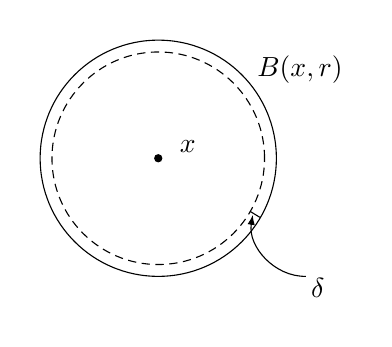
\begin{tikzpicture}[
    scale=1.5,
    background rectangle/.style={fill=white}, show background rectangle]

    \node at (.25,0.1) (x) {$x$};
    % dot at 0,0 with label x
    \fill (0,0) circle (1pt);

    % circle with radius 1cm 
    \draw (0,0) circle (1cm);
    \node at (1.2,.75) (Bxr) {$B(x,r)$};
    % inner circle with radius 0.9cm
    \draw [densely dashed] (0,0) circle (0.9cm);

    % draw a small segment between the two circles on roughly the -30 degree line 
    \draw [solid] (0.778,-.45) -- (.86,-.5);

    % draw an arrow bending up and around from south east of the circle to 
    % label r 
    \draw [-{Latex[length=1.25mm]}] (1.25,-1) to [bend left=50] (.8,-.48);
    \node at (1.35,-1.1) (delta) {$\delta$};
    
\end{tikzpicture}
\end{document}